%---------- Quinto Capitulo ----------
\chapter{Desenvolvimento}
Este trabalho de conclusão de curso necessitou que fosse implementado uma aplicação servidora, o \textit{Broker}, que gerencia a escolha das aplicações que melhor atendem as configurações definidas pelo usuário; a aplicação para dispositivo móvel, onde o usuário realiza as configurações que deseja para cada tipo de serviço e que também consome esses serviços; e também alguns simuladores de provedores de serviços.

\begin{figure}[!htb]
  \centering
  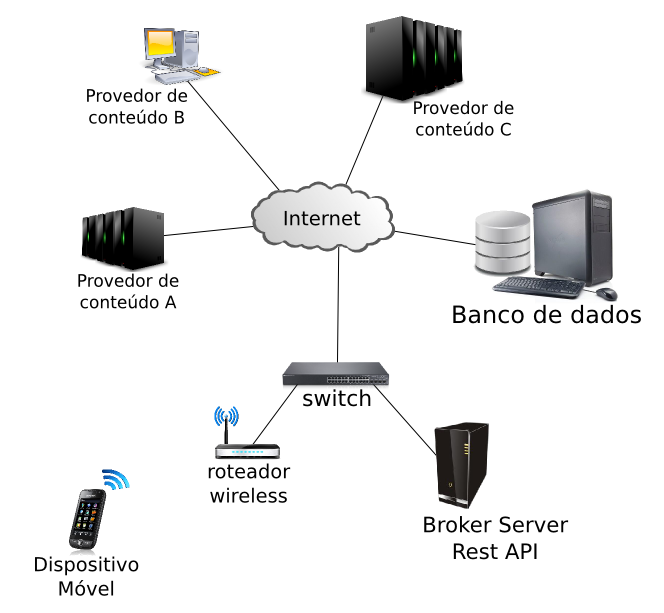
\includegraphics[width=.7\textwidth]{arquitetura.png} % <- formatos PNG, JPG e PDF
  \caption[Arquitetura do projeto]{Arquitetura do projeto}
  \label{fig:arquitetura}
\end{figure}

\section{O \normalfont\itshape Broker}
O \textit{Broker} foi implementado como um \textit{Web Services} \sigla{REST}{Representational State Transfer} que expôe as interfaces necessárias para a aplicação cliente instalada no dispositivo móvel.
\begin{citacao}
O estilo REST é uma abstração dos elementos arquitectônicos dentro de um sistema hipermídia distribuído. REST ignora os detalhes da implementação do componente e da sintaxe do protocolo, a fim de se concentrar nos papéis dos componentes, as restrições sobre a sua interação com outros componentes, e sua interpretação de dados significativos. Ela abrange as restrições fundamentais sobre os componentes, conectores e dados que definem a base da arquitetura Web e, portanto, a essência do seu comportamento como um aplicativo baseado na rede. \cite{fielding2000architectural}
\end{citacao}
Em outras palavras, REST é um alternativa leve para \textit{Web Services} pois ele expõe apenas interfaces com os métodos padrão do \sigla{HTTP}{Hypertext Transfer Protocol}, que também são conhecidos como verbos: GET e POST. Além desses dois existem os PUT, DELETE, HEAD e OPTIONS\footnote{O significado de cada um desses métodos é definido na especificação do HTTP, juntamente com algumas garantias sobre o seus comportamentos}.

As interfaces que o servidor \textit{Broker} expõe aceitam e respondem objetos JSON, como por exemplo uma chamada GET ao método \textit{types} que responde uma lista com os tipos de serviços disponíveis e suas configurações.
Se fizermos essa requisição \url{http://brokerserver.herokuapp.com/types} à API REST, teremos como resultado uma lista de objetos JSON como no exemplo abaixo:
\begin{verbatim}
  [{ "_id": "5605df14e4b0eeb9ac04606c",
     "type": "Weather",
     "icon": "icon ion-ios-partlysunny",
     "url": "#/weather",
     "preferences": [
       { "element": "input",
         "type": "checkbox",
         "name": "last",
         "label": "Last update"
       },{ "element": "input",
         "type": "text",
         "name": "city",
         "label": "City"
       } ]
   },{"_id": "5605df22e4b0eeb9ac04606d",
    "type": "Music",
    "icon": "icon ion-music-note",
    "url": "#/music",
    "preferences": [
      { "element": "input",
        "type": "number",
        "name": "amount",
        "label": "Amount of music"
      } ]
} ]
\end{verbatim}

Já ao realizar o login na aplicação instalada no dispositivo móvel, faremos uma chamada POST ao método \textit{login} do \textit{Broker}, sendo uma chamada POST, os parâmetros irão ser enviados ao servidor no corpo da mensagem, como podemos notar no exemplo abaixo, onde a aplicação foi executada em um navegador de internet com o console de \textit{debug} aberto.

Ao apertar o botão \textit{'Log in'} na aplicação móvel, a \sigla{URL}{Uniform Resource Locator} \url{
http://brokerserver.herokuapp.com/login} foi chamada com os parâmetros \textit{email} e \textit{password} sendo enviados no corpo da mensagem.

\begin{figure}[h]
  \center
  \subfigure[fig:login][\textit{Login} na aplicação do dispositivo móvel]{
\includegraphics[width=7cm]{login.png}}
  \qquad
  \subfigure[fig:debug][\textit{Debug} da aplicação em um navegador de internet]{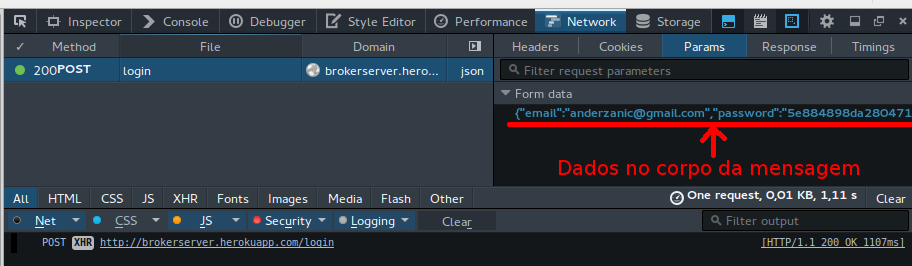
\includegraphics[width=1.1\textwidth]{debug.png}}
  \caption[\textit{Debug} da simulação de um \textit{login} na aplicação móvel]{\textit{Debug} da simulação de um \textit{login} na aplicação móvel}
\end{figure}

\subsection{Plugar novos serviços}
O \textit{Broker} é o sistema encarregado de realizar a análise das preferências do usuário e deve cruzar essas informações com os estados dos provedores de serviço para poder decidir qual é o serviço que melhor atende aos requisitos do usuário.

Dependendo da linguagem de programação escolhida para resolver esse tipo de problema, pode ser que sejam necessárias muitas linhas de código para que seja alcançado um algorítmo adequado.

A característica funcional do Javascript foi um fator relevante pois foram utilizadas funções de alta ordem, funções que podem ser passadas como parâmetros para outras funções, e elas auxiliaram na resolução do problema com um código simples, limpo e elegante. Abaixo temos um exemplo do uso de funções de alta ordem em Javascript.

Suponha que temos uma lista de objetos e é preciso escolher um desses objetos, em Javascript podemos implementar uma função que funcionará como um predicado, e todos os objetos que responderem \textit{"verdade"} a esse predicado, serão escolhidos.

\begin{verbatim}
    var lista = [ {"cidade": "Maringá", "Estado":"PR"},
                  {"cidade": "Curitiba", "Estado":"PR"} ];
    var predicado = function(candidato){
                      return candidato.cidade === "Maringá";
                    };
    var resultado = lista.filter(predicado);
    console.log(resultado);
    // Imprime no console: [{"cidade": "Maringá", "Estado":"PR"}]
\end{verbatim}

Esse é um exemplo bem simples, mas a função de predicado pode ter a complexidade necessária e ainda assim o código que aplica o predicado se manterá sempre simples e além disso essa função poder ser modularizada transformado-se em um \textit{plugin} que poderá ser aplicado onde for necessário.

No caso do \textit{Broker} isso foi fundamental pois cada vez que um novo serviço for ser oferecido será apenas necessário implementar o predicado, baseado nos atributos do serviço, e realizar o registro desse novo predicado no servidor, com a adição de uma única linha de código:
\begin{verbatim}
    var novoservico = require('./novoservico.js');
\end{verbatim}

\subsection{Jasmine \normalfont\itshape Framework}
Jasmine é um \textit{framework} para testes de códigos Javascript.
\begin{citacao}
Jasmine é um framework de testes \sigla{BDD}{Behavior Driven Development} para JavaScript. Ele não depende de navegadores, \sigla{DOM}{Document Object Model}, ou qualquer \textit{framework} JavaScript. Jasmine é adequado para websites, projetos Node.js, ou em qualquer lugar que o JavaScript possa ser executado.\cite{jasmine}
\end{citacao}

Como Javascript é uma linguagem de tipagem dinâmica, é necessário que sejam implementados testes que possam aumentar a confiança de que as funções estão respondendo de maneira correta.
Dessa forma, algumas funções do \textit{Broker} tiveram testes implementados.

O \textit{framework} Jasmine suporta a técnica ágil "Desenvolvimento Guiado por Comportamento", conhecido pela sigla em inglês BDD, é uma técnica que encoraja o envolvimento entre os desenvolvedores, setores de qualidade e pessoas sem conhecimento técnico e que dominam a regra do negócio. Os testes são criados utilizando a linguagem nativa e a codificação do teste em Javascript, o uso da linguagem nativa auxilia o desenvolvedor a manter o foco na razão pela qual o código deve ser implementado.
Abaixo temos um exemplo de um teste com Jasmine:
\begin{verbatim}
describe("serviços disponíveis", function() {
  beforeEach(function() {
    jasmine.Ajax.install();
    jasmine.Ajax.stubRequest('http://weather-provider.herokuapp.com/weather')
      .andReturn({
        responseText: { "provider": "Weather Provider",
                        "city": "Maringá",
                        "temperature": 29,
                        "Humidity": 48,
                        "sky": "weather-sunny",
                        "update": "2016-02-10T18:23:44.479Z" };
      });
  });
  afterEach(function() {
    jasmine.Ajax.uninstall();
  });
  it("a temperatura de Maringá deverá ser exibida", function() {
    $.ajax({
      url: 'http://weather-provider.herokuapp.com/weather'
    }).success(result){
      expect(result.city).toEqual('Maringá');
      expect(result.temperatura).toEqual(29);
    };
  });
});
\end{verbatim}
Antes da execução de cada teste, que está implementado dentro de cada declaração "it('mensagem', function(){});", é executado o código declarado na função 'beforeEach'. Isto cria um ambiente que responderá às chamadas Ajax no endereço 'http://weather-provider.herokuapp.com/weather' com a resposta declarada em 'responseText'.

No final da execução de cada teste o trecho 'afterEach' é executado destruindo o ambiente criado.

Esses ambientes são conhecidos como \textit{Mocks} e servem para isolar o teste no que realmente deve ser testado, no caso do exemplo, se a chamada Ajax não fosse um ambiente falso, ela tentaria realizar uma requisição, isso dependeria de conexão à internet, do endereço que está sendo chamado ter um servidor ativo. São muitas variáveis a serem controladas e desnecessárias para um teste unitário.
\section{A aplicação para dispositivos móveis}
A implementação do aplicativo para dispositivo móvel utilizou o Ionic \textit{Framework}. Dessa forma, a aplicação foi desenvolvida com o uso das Linguagens Javascript, HTML e CSS.

O Ionic \textit{Framework} foi desenvolvido sobre outro \textit{framework}, o Apache Cordova, o que idealmente permite que a aplicação desenvolvida possa ser executada em todas as plataformas de dispositivo móvel à qual o Apache Cordova oferece suporte.

Abaixo é apresentada a figura \ref{fig:ionicarch} que demonstra a organização da arquitetura do \textit{framework}. Essa figura é meramente ilustrativa, pois nas últimas camadas temos um número bem maior de funcionalidades nos dispositivos, assim como um número maior de sistemas operacionais alvos do Apache Cordova.

\begin{figure}[!htb]
  \centering
  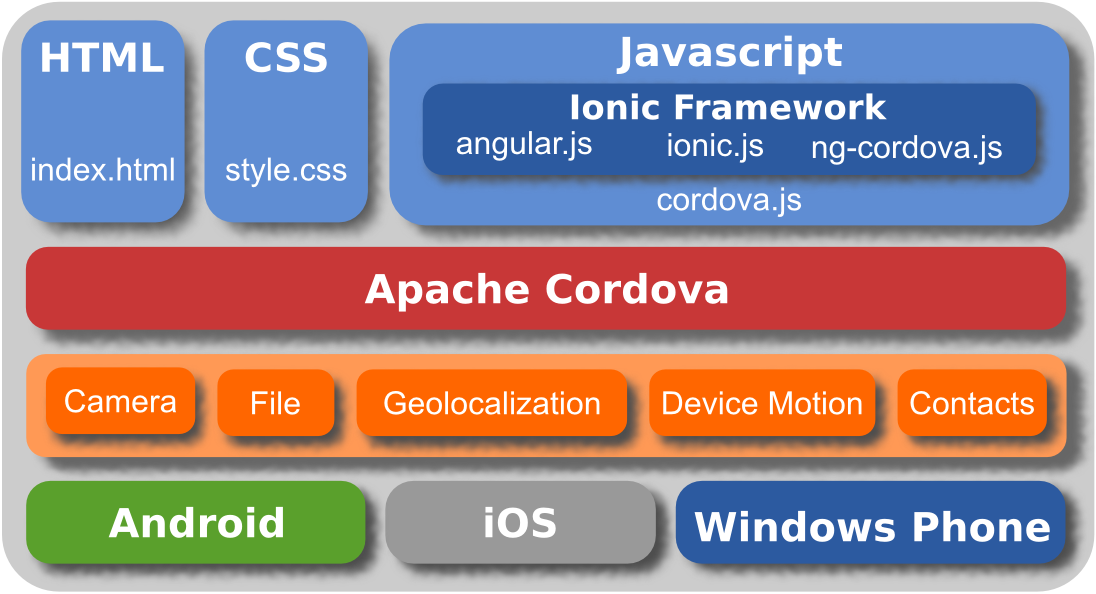
\includegraphics[width=.8\textwidth]{ionicarch.png} % <- formatos PNG, JPG e PDF
  \caption[Arquitetura do Ionic Framework]{Arquitetura do Ionic Framework}
  \label{fig:ionicarch}
\end{figure}

A implementação e os testes da aplicação tiveram como SO alvo apenas o Android.

A aplicação foi desenvolvida com uma interface intuitiva, com ícones expressivos para que o usuário tivesse uma experiência agradável e sem transtornos.

As configurações necessárias são mínimas e qualquer pessoa envolvida no contexto da aplicação conseguiria realizá-las em poucos passos e já teria a aplicação em funcionamento em seu aparelho.

O Anexo A apresenta um modelo de navegação na aplicação.

\subsection{Angular.js}
Angular.js foi desenvolvido pelo Google. É um \textit{framework} para desenvolvimento de aplicações web \textit{Single Page Applications}, onde todas as páginas da aplicação são desenvolvidas como \textit{templates} e são injetadas na página principal quando requisitadas.

Uma característica muito importante do Angular.js é que ele extende o vocabulário padrão do HTML, permitindo que sejam desenvolvidos sistemas com um código muito mais expressivo no \textit{front-end}.

Como por exemplo o uso de uma \textit{tag} HTML como: 
\begin{verbatim}
                <genero />
\end{verbatim}

é mais expressivo do que:
\begin{verbatim}
                <label>Gênero: </label>
                <select name="genero">
                  <option value="M">Masculino</option>
                  <option value="F">Feminino</option>
                </select>
\end{verbatim}

Além desse ganho na expressividade, a modularização e reuso de código acontece efetivamente, o que diminui o tempo de desenvolvimento e aumenta a qualidade das aplicações.

Outro recurso muito interessante é o \textit{Two-Way Data Binding}, que permite a sincronização automática dos dados da \textit{view} com o modelo sem a manipulação direta do DOM pelo desenvolvedor.

\begin{figure}[!htb]
  \centering
  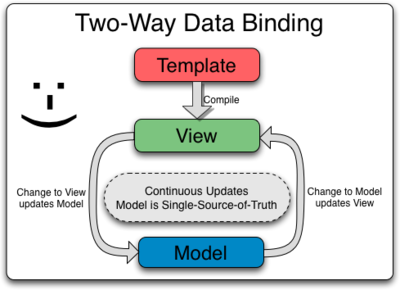
\includegraphics[width=.6\textwidth]{databinding.png} % <- formatos PNG, JPG e PDF
  \caption[Sincronização automática do \textit{model} e da \textit{view}]{Sincronização automática do \textit{model} e da \textit{view}}
  \label{fig:twoway}
\end{figure}

\subsection{Construção dinâmica de formulário}
Um dos desafios enfrentado durante a implementação da aplicação para o dispositivo móvel foi a construção do formulário que exibe as configurações das preferências do usuário para cada serviço. Como cada serviço apresenta um determinado conjunto de atributos, iria ser necessário a implementação de uma \textit{template} para cada tipo de serviço, isso iria aumentar a complexidade de atualizações e manutenções de código.

Para evitar esses problemas e outros que poderiam surgir, como por exemplo: uma mudança nos atributos do serviço, foi desenvolvido um componente, que constroe o formulário de configuração de preferências de acordo com parâmetros enviados pelo \textit{Broker}.

Por exemplo, podemos enviar essas configurações abaixo ao dispositivo móvel e ele produzirá um formulário como a figura \ref{fig:geracaoauto}
\begin{verbatim}
        { "element": "input",
          "type": "text",
          "name": "email",
          "label": "Email"
        },
        { "element": "input",
          "type": "password",
          "name": "password",
          "label": "Password" }
\end{verbatim}

\begin{figure}[!htb]
  \centering
  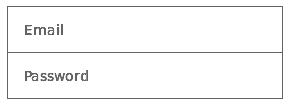
\includegraphics[width=.5\textwidth]{geracaoauto.png} % <- formatos PNG, JPG e PDF
  \caption[Geração automática de formulário]{Geração automática de formulário}
  \label{fig:geracaoauto}
\end{figure}

\section{Ferramentas}
\subsection{MongoLab}
O banco de dados utilizado foi o MongoDB, e como SGDB foi escolhido o MongoLab.
O MongoLab pode ser acessado através do endereço \url{http://mongolab.com} é um serviço de banco de dados online que oferece diversos pacotes de soluções para MongoDB com diversos preços, desde o pacote gratuito com algumas restrições de uso até pacotes com valores de USD 5890.00.

O MongoLab oferece recursos para a manipulação e gerenciamento dos dados através de:
\begin{itemize}
\item uma interface web;
\item chamadas à API REST;
\item conexões por \textit{driver};
\end{itemize}

Para o \textit{Broker} foi configurado o uso de \textit{driver} de conexão, pois ele apresenta o melhor desempenho das opções existentes.

\subsection{Heroku}
Heroku é um serviço de hospedagem de aplicações que também possue os pacotes gratuito e pagos. A forma de cobrança do Heroku é diferente, a cobrança acontece de acordo com o uso de processamento e requisições de suas aplicações.

Ele possui uma aplicação cliente que permite monitorar e controlar suas aplicações, além da interface web que também permite o controle das aplicações.

Uma funcionalidade muito interessante do Heroku é a integração com o GitHub que permite o \textit{deploy} automático das aplicações assim que as alterações são versionadas em uma determinada \textit{branch}.

\subsection{GitHub}
O Git foi escolhido como o sistema de controle de versão das aplicações móvel e servidora e até deste documento. E o GitHub foi o escolhido como plataforma de hospedagem.
O GitHub permite a criação gratuita de repositórios públicos e possui ferramentas na plataforma web que permitem gerenciar e monitorar os repositórios.
Na lista abaixo temos os endereços dos repositórios que podem ser clonados:

\begin{itemize}
\item[TCC:] \url{https://github.com/andersonzanichelli/tcc-informatica.git}
\item[Broker:] \url{https://github.com/andersonzanichelli/brokerserver.git}
\item[Cliente:] \url{https://github.com/andersonzanichelli/brokerclientapp.git}
\end{itemize}

\subsection{NPM e Bower}
Assim como as aplicações Java contam com o Maven ou Gradle como ferramentas de gerenciamento de dependências, Javascript tem o \sigla{NPM}{Node.js Package Manager}. Para dependências de \textit{front-end} foi utilizado o Bower.
Gerenciadores de dependências são ferramentas incríveis que configuram um ambiente de desenvolvimento, de teste ou de produção automaticamente e de forma padronizada, com as versões corretas de cada dependência.